\documentclass[11pt]{article}

\usepackage[utf8]{inputenc}
\usepackage[T1]{fontenc}
\usepackage[head=26pt, a4paper, margin=1.2in, top=1.4in, bottom=1.75in]{geometry}
\usepackage{fancyhdr}
\usepackage{lastpage}
\usepackage[hidelinks, colorlinks, urlcolor=blue, linkcolor=black,citecolor=magenta]
{hyperref}
\usepackage{amsmath}
\usepackage{amsthm}
\usepackage{amssymb}
\usepackage{graphicx}
\usepackage{float}
\usepackage{listings}
\usepackage{mathtools}
\usepackage{enumitem}


\usepackage{indentfirst}
\usepackage{a4wide}
\usepackage{color}
\usepackage{lipsum}
\usepackage{multicol}
\usepackage{tikz}
\usetikzlibrary{arrows,shapes,positioning}

% ---------------- Page and margin/header/footer Setup -----------------
\pagestyle{fancy}
%\fancyhf{} % Clears header and footer
\fancyhead{}
\fancyfoot{}
\lhead{ACS --- Assignment 2}
\rhead{DIKU}
\lfoot{Page \thepage\ of \pageref{LastPage}}
\rfoot{Nicolai Jørgensen \\ Yiran Zhang}
\renewcommand{\headrulewidth}{0.4pt}
\renewcommand{\footrulewidth}{0.4pt}
% ----------------------------------------------------------------------

\newtheorem{mythm}{Theorem}
\newtheorem{mydef}{Definition}

\DeclarePairedDelimiter{\ceil}{\lceil}{\rceil}
\newcommand\numberthis{\addtocounter{equation}{1}\tag{\theequation}}

\newcommand{\HRule}{\rule{\linewidth}{0.5mm}}

\title          {Assignment 2}
\author         {Nicolai Jørgensen and Yiran Zhang}

\begin{document}

\maketitle
\newpage

\section{Question 1}

\begin{enumerate}
	\item
     the precedence graph for each schedule are showing below , these two schedules are conflict- 
     serializable, because their the precedence graph are acyclic.
		
		\begin{figure}[H]
			\centering
			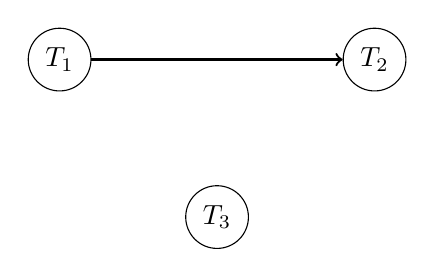
\begin{tikzpicture}
			[task/.style={circle, draw},] 
          	\node[task] (T1) at (0.0, 2.0) {$T_1$}; 
          	\node[task] (T2) at (4.0, 2.0) {$T_2$}; 
          	\node[task] (T3) at (2.0, 0) {$T_3$}; 
           
            \draw[->, thick, draw] (T1.east) to [out=0,in=180] (T2.west); 
			\end{tikzpicture} 

			\caption{Precedence graph for schedule 1} 
			\label{fig:trans-schedule-1} 
		\end{figure}

		\begin{figure}[H]
			\centering
			\begin{tikzpicture}
			[task/.style={circle, draw},] 
          	\node[task] (T1) at (0.0, 2.0) {$T_1$}; 
          	\node[task] (T2) at (4.0, 2.0) {$T_2$}; 
          	\node[task] (T3) at (2.0, 0) {$T_3$};  
           
			\end{tikzpicture} 

			\caption{Precedence graph for schedule 2} 
			\label{fig:trans-schedule-1} 
		\end{figure}		
		
	\item
	The \textbf{schedule 1} couldn't have been generated by a scheduler using strict two-phase locking 
	(strict 2PL), because there is a read lock in X in $T_1$, and then $T_2$ want to set a write lock on 
	X, it must wait for until $T_1$ release the read lock.
	
	The \textbf{schedule 2} could have been generated by a scheduler using strict two-phase locking 
	(strict 2PL), because there	
		
		
\end{enumerate}

\section{Question 2}

\begin{enumerate}
		\item
		T3 must be rolled back. 
			\begin{itemize}
				\item
				test1 fails, because T2 not completes before T3 starts.
				\item
				test2 fails, because T2 completes before T3 begins with its write phase. but the 
				WriteSet(T2) $\cap$ ReadSet(T3) is not empty, and the offending object is 4.
				\item
				test3 fails, no one meets the conditions of test3
			\end{itemize}
		
		\item
		T3 must be rolled back. 
			\begin{itemize}
				\item
				test1 fails, because no one meets the conditions of test1
				\item
				test2 fails, because T1 completes before T3 begins with its write phase. but the 
				WriteSet(T1) $\cap$ ReadSet(T3) is not empty, the offending object is 3.
				\item
				test3 fails, because T1 doesn't meets the conditions of test3.
			\end{itemize}				
		
		\item
		T3 is allowed to commit, test2 is necessary to reach the conclusion. T1 completes before T3 
		begins with its write phase, and the WriteSet(T1) $\cap$ ReadSet(T3) is empty. T2 completes 
		before T3 begins with its write phase, and the WriteSet(T2) $\cap$ ReadSet(T3) is empty.			
	
\end{enumerate}
 
\section{Question 3}
\begin{enumerate}
	\item
		\begin{itemize}
		 \item[a)]
		 \begin{itemize}
		 \item
		 For \textit{SingleLockConcurrentCertainBookStore}, first we take \textbf{writeLock} on data 
		 items that are modified and take \textbf{readLock} on data items that are read, then execute 
		 transaction, finally release all locks. Therefore each newly created transaction \textit{i} 
		 must, before reading or writing any data, waiting until the preceding transaction has either 
		 committed or aborted. The scheme forces all transactions to execute in the serial order. 
		 Since that order is a possible serial order of the various transaction, by definition simple 
		 serialization will produce transactions that are serialized and thus are correct before-or-
		 after actions.
		 
		 \item
		 For \textit{TwoLevelLockingConcurrentCertainBookStore}, at top-level the
		 \textbf{takeGlobalLock} is acquired on exclusive mode when we perform \textbf{addBooks} and 
		 \textbf{removeBooks}, \textbf{globalReadLock} is in all the other operations. This scheme is 
		 also the scheme on \textit{SingleLockConcurrentCertainBookStore}, thus at top level we 
		 achieve correct before-or-after atomicity.
		 
		 At the bottom level, there is one read-write lock for each book in the bookstore.
		 \textbf{takeLocalWriteLock} on data items that are modified and \textbf{takeLocalReadLock} on 
		 data items that are read, but do this during execution of transaction (as needed). Release 
		 locks on objects no longer needed during execution of transaction. This solution can also 
		 forces all the transaction at bottom level to execute in serial order. 
		 
		 At each level the transactions are executed in serial order, so the  
		 \textit{TwoLevelLockingConcurrentCertainBookStore} has the correct before-or-
		 after actions.
		\end{itemize}
		
		\item[b)]
		\textbf{Test 1} tests that concurrently adding copies and buying books maintain consistent 
		state. We initiate the number of copies of the default book. Two threads C1 and C2 run 
		concurrently and iterate buyBooks and addCopies 10000 times  respectively. We finally check 
		whether the finally value is equivalent to the initial value. When we take write or read lock 
		on the data items the final value is equal to the initial value, otherwise the final value 
		varies. The anomalies occurs if the final value varies, in this case, buyBooks happens during 
		the addCopies or the addCopies happens during the buyBooks, and this will lead to dirty reads 
		or dirty writes and make the final value to vary.
		
		\item[c)]
		We don't have to consider different testing. Because the scheme in the \textit{SingleLockConcurrentCertainBookStore},  is the same as the scheme in the top-level in the \textit{TwoLevelLockingConcurrentCertainBookStore}
		
		The use of different strategies would not be a violation of modularity.
		\end{itemize}
	\item
	\item
		\begin{itemize}
		 \item
		 For \textit{SingleLockConcurrentCertainBookStore}, our locking protocol will not lead to 
		 deadlocks. We first take \textbf{writeLock} on data items that are modified and take 
		 \textbf{readLock} on data items that are read, then execute transaction, finally release all 
		 locks. Therefore there is no deadlocks.
		 
		 \item
		 For \textit{TwoLevelLockingConcurrentCertainBookStore}, our locking protocol will lead to 
		 deadlocks. At top-level the \textbf{takeGlobalLock} is acquired on exclusive mode when we 
		 perform \textbf{addBooks} and \textbf{removeBooks}, \textbf{globalReadLock} is in all the 
		 other operations. At the bottom level, there is one read-write lock for each book in the 
		 bookstore.
		 \textbf{takeLocalWriteLock} on data items that are modified and \textbf{takeLocalReadLock} on 
		 data items that are read, but do this during execution of transaction (as needed). Release locks 
		 on objects no longer needed during execution of transaction. Therefore we need to know when to 
		 release locks, which may leads to deadlocks.
	
		\end{itemize}
	
\end{enumerate}

\end{document}
